\documentclass[10pt,a4paper, titlepage, toc=idx]{scrreprt}

\usepackage[english]{babel}
\usepackage[utf8]{inputenc}
\usepackage{amsmath, amsthm, amssymb, amsfonts}
\usepackage{enumitem}
\usepackage{calrsfs}
\usepackage{mathtools}
\usepackage{mathrsfs}
\usepackage{nicefrac}
\usepackage{stmaryrd}
\usepackage{wasysym}
\usepackage{pifont}
\usepackage{wrapfig}

\usepackage{listings}

\usepackage{color}

\definecolor{mygreen}{rgb}{0,0.6,0}
\definecolor{mygray}{rgb}{0.5,0.5,0.5}
\definecolor{mymauve}{rgb}{0.58,0,0.82}

\lstset{ %
	backgroundcolor=\color{white},   % choose the background color; you must add \usepackage{color} or \usepackage{xcolor}
	basicstyle=\footnotesize\ttfamily,        % the size of the fonts that are used for the code
	breakatwhitespace=false,         % sets if automatic breaks should only happen at whitespace
	breaklines=true,                 % sets automatic line breaking
	captionpos=b,                    % sets the caption-position to bottom
	commentstyle=\color{mygreen},    % comment style
	columns=fixed
	deletekeywords={...},            % if you want to delete keywords from the given language
	escapeinside={\%*}{*)},          % if you want to add LaTeX within your code
	extendedchars=true,              % lets you use non-ASCII characters; for 8-bits encodings only, does not work with UTF-8
	frame=single,                    % adds a frame around the code
	keepspaces=true,                 % keeps spaces in text, useful for keeping indentation of code (possibly needs columns=flexible)
	keywordstyle=\color{blue},       % keyword style                 % the language of the code
	language=bash,
	morekeywords={*,...},            % if you want to add more keywords to the set
	numbers=none,                    % where to put the line-numbers; possible values are (none, left, right)
	numbersep=5pt,                   % how far the line-numbers are from the code
	numberstyle=\tiny\color{mygray}, % the style that is used for the line-numbers
	rulecolor=\color{black},         % if not set, the frame-color may be changed on line-breaks within not-black text (e.g. comments (green here))
	showspaces=false,                % show spaces everywhere adding particular underscores; it overrides 'showstringspaces'
	showstringspaces=false,          % underline spaces within strings only
	showtabs=false,                  % show tabs within strings adding particular underscores
	stepnumber=1,                    % the step between two line-numbers. If it's 1, each line will be numbered
	stringstyle=\color{mymauve},     % string literal style
	tabsize=2,                       % sets default tabsize to 2 spaces                  % show the filename of files included with \lstinputlisting; also try caption instead of title
	%	linewidth=80em,
}

\lstset{prebreak=\raisebox{-1ex}[0ex][0ex]
	{\ensuremath{\hookleftarrow}}}
\lstset{postbreak=\raisebox{0ex}[0ex][0ex]
	{\ensuremath{\hookrightarrow\space}}}

%\usepackage{lastpage}
\usepackage[svgnames]{xcolor}

%\usepackage{skriptum} % Layout and Design
% don't change the order of these or \i won't work as it should (I don't see why but that's how it is)
%\usepackage{cscallr} % Macros

\usepackage[T1]{fontenc}

\usepackage{charter}
\usepackage[bitstream-charter]{mathdesign} % imo nicer looking math font (fitting to the text font)
%\usepackage[expert]{mathdesign} % standard math font
\renewcommand*{\descfont}{\usefont{T1}{qhv}{b}{n}} 
\usepackage{fancyhdr, hyperref, titlesec, blindtext, color, subfigure}

%\usepackage{sectsty}
%\chapterfont{\usefont{T1}{bch}{b}{n}\selectfont\huge}

\hypersetup{hidelinks, linktoc=all,}

\newcommand{\HRule}{\rule{\linewidth}{0.5mm}}

\fancyhead[L]{\leftmark}
%\fancyhead[R]{\rightmark}
\fancyhead[R]{}
\fancyfoot{}
%\fancyfoot[L]{\emph{Skriptum Lineare Algebra I}} % name
\fancyfoot[C]{\thepage}
%\fancyfoot[R]{\emph{WS 2013/2014}} % semester
\pagestyle{fancy}
%headers
\renewcommand{\chaptermark}[1]{\markboth{\textsc{\chaptername\ \thechapter.\ #1}}{}}
\renewcommand{\sectionmark}[1]{ \markright{#1}{} }

% TOC
\usepackage[subfigure]{tocloft} % subfigure option only if using subfigure package
\renewcommand{\cfttoctitlefont} % ToC title
{\usefont{T1}{qhv}{b}{n}\selectfont\huge}
\renewcommand{\cftchapfont} % chapter titles
{\usefont{T1}{qhv}{b}{n}\selectfont}
\renewcommand{\cftsecfont} % section titles
{\usefont{T1}{bch}{m}{n}\selectfont}
\renewcommand{\cftsubsecfont} % subsection titles
{\usefont{T1}{bch}{m}{n}\selectfont} 
\renewcommand{\cftchappagefont} % chapter page numbers
{\usefont{T1}{bch}{b}{n}\selectfont}
\renewcommand{\cftsecpagefont} % section page numbers
{\cftsecfont} 
\renewcommand{\cftsubsecpagefont} % subsection page numbers
{\cftsubsecfont}

% chapter
\definecolor{gray75}{gray}{0.75}
\newcommand{\hsp}{\hspace{20pt}}
\titleformat{\chapter}[hang]{\Huge\fontfamily{qhv}}{\fontfamily{qhv}\bfseries\thechapter\hsp\textcolor{gray75}{$\vert$}\hsp}{0pt}{\Huge\bfseries}
% section
\titleformat{\section}[hang]{\Large\bfseries\fontfamily{bch}}{\thesection}{10pt}{\bfseries}
%subsection
\titleformat{\subsection}[hang]{\bfseries\fontfamily{bch}}{\thesubsection}{5pt}{\bfseries}

% theorems, not used in the linear algebra I script yet
\theoremstyle{definition}
\newtheorem{deff}{Definition}[section]
\theoremstyle{plain}
\newtheorem{propp}{Proposition}[section]

% macros
\renewcommand\over[2]{\genfrac{}{}{0pt}{}{#1}{#2}}

\newcommand*{\product}{Grit}
\newcommand*{\version}{1.1}
\newcommand*{\website}{\url{team-grit.com}}
\newcommand*{\repo}{\url{github.com/team-grit/grit}}


\begin{document}
%	\tikzstyle{every picture}+=[remember picture]
% \input{title.tex}
\begin{titlepage}
  \begin{center}
			
    % Upper part of the page. The '~' is needed because \\
    % only works if a paragraph has started.
    % \includegraphics[width=0.3\textwidth]{title_pic}~\\[1cm]
			
    % \textsc{\LARGE Grit}\\[1.5cm]
    
\includegraphics{pictures/grit}
			
    % Title
    \HRule \\[0.4cm]
    {\fontfamily{qhv} \huge \bfseries Using the\\\product{} Submission
      System \\[0.4cm] }
			
    \HRule \\[.5cm]
			
			
    {\small Official User Manual for Version \version}\\[1.5cm]
			
    
\includegraphics[scale=.25]{pictures/1024}
			
    % Author and supervisor
    % \begin{minipage}{0.4\textwidth}
    %   \begin{flushleft}
    %   \end{flushleft}
    % \end{minipage}
    % \begin{minipage}{0.4\textwidth}
    %   \begin{flushright}
    %     \large
    %     \emph{gelesen von:} \hfill
    %     Prof. Dr. Markus \textsc{Schweighofer}\\
    %   \end{flushright}
    % \end{minipage}
    % \large
    % \emph{Autor:} \hfill
    % Thomas \textsc{Schmidt}
			
    \vfill
			
    % Bottom of the page
    % {\large Sommesemester 2014}\\
    {\large \today}
			
  \end{center}
\end{titlepage}
\setcounter{tocdepth}{1}
	
\setcounter{page}{2} \cleardoublepage
\tableofcontents
\chapter{What is \product?}
%	\product{} offers a comprehensive solution for submission,
% fetching, evaluating and processing of programming course
% submissions. All you have to do is to press one button. The
% server-application constantly keeps an eye on associated
% repositories, e.g. \textsc{Ilias} and SVN, intelligently fetches
% student-submitted code and runs predefined tests. In the end, you
% receive a well-formatted PDF document or a plain-text file
% containing all the submissions of one assignment ready to print and
% hand over
% to your correctors.\\
%	Furthermore, \product{} lets you create overall statistics on
% score for one assignment, as well as for entire courses. Thus, it is
% easy to keep track on how your students perform.
\product{} is a system, developed by {\sc Team
  Grit} and improved by {\sc Team Varcid}, that makes the life of lecturers and
tutors of mainly programming courses easier and more comfortable. With
\product, we implemented a server-side one-button solution for
fetching and processing student submissions. This is done in such a
way that the tutors will not have to worry about not-compiling
programs and can therefore concentrate on the actually written code
and its quality. \product{} helps to maximize the teaching quality by
ruling out unnecessary work and lets the tutors focus on the really
important matter: Teaching.
\section{What does \product{} do?}
With \product, the students do not directly submit their solutions to
our application. To be precise, they will not even notice that you are
using \product{} when submitting. Rather, \product{} fetches the student
submissions from whatever system provided for that purpose. As for
now, \product{} supports Subversion, and Email submissions,
however, because of its high modularity, you can easily add your own
{\it fetcher}. At the end of a previously set deadline,
\product{} fetches the submissions and processes them. As of now, we
support Java, C and Haskell submissions, but like {\it fetchers},
additional modules can be added. After the processing, which includes
compiling and testing the submission, using previously set unit tests,
we will put that acquired information about the submission in a
report, ready for you to download. For now that report will be either
a PDF or a plain-text file, but, as you will have guessed, other
formats can be implemented easily.
\subsection*{What \product{} does not.}
\product{} does not provide submission features, as it can only import
submissions. Also, it is not possible to manipulate code in \product,
because this is not what it was intended for: offline correction on
paper.  \product{} does not replace a lecturer or tutor by adopting all
of their correction procedure, however \product{} simplifies their work
in supporting them with automatable checking routines. So,
\product{} does not offer any methods to control semantical errors in
the program code like checking if the summation really does add the
two summands.  Furthermore \product{} is not suitable to test if the
submitted solutions of the students actually solves the given problem or
a part of it. \product{} cannot check any additional exercise
restrictions specified in the assignment paper (e.g. using inherited
methods for solving the exercise). \product{} will also not correct any
programming faults automatically, but will present you the incorrect
passage, the error, the passed tests as well as compiler
error message.
\section{When do you need \product?}
You are a lecturer/tutor of a general programming course, a java
workshop, a C++ seminar, ..., in which the participants can or have to
submit solutions to a given problem. If you are tired of searching for
syntax errors, compiling errors, typos, etc. for hours at a time, then
you will definitely appreciate our product to increase the efficiency
of your correction by prechecking every submitted solution. All in
all, if you are a university or college professor or lecturer,
teacher, tutor, or corrector, \product{} can help you automate
collecting electronically submitted assignments concerning programming
code from various resources. Compiling tests and predefined tests can
be run so you can easily focus on the important things.

\subsection*{When you do not need \product.}
You will not need \product{} if you do not provide electronic submission of
assignments for your course. Also, \product{} is only suitable for
fetching programming code assignments, however, other types of
submissions can be added by oneself.  \product{} does not offer any
features for students, as it only provides functionalities used by
teachers and correctors.
\section{What are the alternatives?}
\textsc{Team Varcid} has compared \product{} with the following alternatives. You can find it in another document.
\begin{itemize}
\item The Marmoset Project \\
  (\url{marmoset.cs.umd.edu}) \\
  Marmoset is a system for handling student programming project
  submission, testing and code review. It has been developing at the
  University of Maryland for over 5 years. It works in all different
  programming languages, and is designed to work well with both very
  small and very large projects, such as our OS course in which a
  submission consists of tens of thousands of lines of code.
\item BOSS Online Submission System (Beta phase) \\
  (\url{sourceforge.net/projects/cobalt}) \\
  BOSS is a course management tool that allows students to submit
  assignments on-line in a secure manner. Staff can mark work and run
  automatic tests on submissions.
\item Cafe grader \\
  (\url{gitorious.org/cafe-grader}) \\
  Cafe grader is a submission and grading system for programming
  contest and training.  This software was used in APIO'08. It
  currently has mainly two components: the web submission system and
  the grader. The web app uses Ruby on Rails; while the grader was
  written in plain Ruby. Current activity: process of migrating to
  git, and developing installation scripts.
\item Praktomat \\
  (\url{https://github.com/KITPraktomatTeam/Praktomat/})
  \\
  Praktomat is a quality control system for programming
  exercises. Students hand in their submissions directly into
  Praktomat which then compiles and tests them. It was first developed
  at the University of Passau in 1998 and was later migrated to the
  Karlsruhe Institute of Technology in 2008.  The software is written
  in Python and uses the Django web framework. It is able to manage
  Java, other programming languages can be added.
\end{itemize}
% writing modules yourself or using other software
\chapter{Getting Help}
	There are various resources available to get the most out of \product. 
	\section{Online Documentation}
	The online version of the documentation is essentially the
	same as the one you are reading now, however, you will have
	access to additional resources concerning troubleshooting.
	But online you will find the newest version.
	\section{Contact us}
	Do you have suggestions? Do you miss a feature? Contact {\sc Team Grit} or {\sc team Varcid} by mail. 
	You will find our mail addresses at the end of the document.
\chapter{Getting \product}
As you are reading this documentation now, you have most
likely already acquired \product. It is either directly
available by getting it from the developers, or found on the associated
GIT repository, or found on the associated GIT repository.\\

%for questions about vagrant contact team Grit or VARCID
\noindent Fundamental there are two ways to install \product . 
\begin{itemize}
\item direct on a Linux server system
\begin{itemize}
\item with our installation script
\item by hand 
\end{itemize}
%\item[2.] or by vagrant on a virtual machine (for developer or if you use another operation system)
\end{itemize}


\section{Required Software}\label{3.1} For installing \product{} you need the current version of the following software.\\
\noindent The packages will also be installed with the installation script (see \ref{3.2}).
\begin{itemize}
%\item Java Runtime Environment (jre)
\item Java Development Kit (\texttt{jdk7} or higher)\\
		- The package contains the javac compiler, which you need to compile the students' Java submissions
\item \TeX  live (\texttt{texlive-full})\\
		- you need Texlive to create your reports
\item GNU-C-Compiler (\texttt{gcc})\\
		- to compile the students' C submissions
\item Glasgow Haskell Compiler (\texttt{ghc})\\
		- to compile the students' Haskell submissions
\item Subversion (\texttt{svn})\\
		- \product{} can fetch submissions from subversion, 
\item Secure Copy (openssh server and client)
\item G++ Compiler (\texttt{g++})
\item Git\\
		- you need Git to get \product.
\item Gradle\\
		- you need Gradle to install \product.
\end{itemize}
%For developing you also need the following software. For more information see the developer's manual.
%\begin{itemize}
%\item Vagrant (just for virtual machine version)
%\item VirtualBox (just for virtual machine version)
%\end{itemize}

\section{Using installation script}\label{3.2}
\textbf{Warning:} you need a Linux system with apt-get to use the script for a direct installation!\\

\noindent You have to take the script install-GRIT.sh and put it at the place, where \product{} shall be installed. The required software will be installed by the script! Now you have to run script.\\

\noindent For Ubuntu  the next step is to define the rights:
\begin{lstlisting}
	chmod u+x install-GRIT.sh
\end{lstlisting}
and run the installation script:
\begin{lstlisting}
	./install-GRIT.sh
\end{lstlisting}
\product{} should now be installed in a folder ./grit/build/install/GRIT
relative to the directory where you run the install script.

\section{Direct installation (by hand)}
\textbf{Warning:} you need a Linux system to do a direct installation because Grit uses Unix shell commands.\\

\noindent The first step is to install all required files which are listed in \ref{3.1}. Next thing to do is to select the location where grit should be installed. Then you have to generate a git clone in to this location: 
\begin{lstlisting}
	$ git clone https://github.com/VARCID/grit.git
\end{lstlisting}

\noindent Now there should be a folder called grit. You have to go inside the folder:
\begin{lstlisting}
	$ cd grit
\end{lstlisting}

\noindent In the next step you have to run gradlew: 
\begin{lstlisting}
%	$ ./gradlew	NOTE: not needed			
	$ ./gradlew install
\end{lstlisting}
\product{} should now be installed in a folder ./grit/build/install/GRIT
relative to the directory where you run gradlew install.


%NOTE this is now in chapter{Runnning Grit}/section{How to run Grit}
%     as it is not installation by hand specific
%
%\noindent In the Folder grit/build/install/GRIT you will find a file called runscript.sh.
%This file you have to run
%\begin{lstlisting}
%	$ ./runscript.sh
%\end{lstlisting}

%\section{Vagrant VM}
%TODO !!
%Für Win7: putty, VirtualBox, Vagrant
%über cmd: Pfad zu Grit suchen, dann Vagrant up
%Dann installiert er Ubuntu-files
%Dann über putty mit SSH-Client auf Vagrant zugreifen (Vagrant gibt einem die ip an)
%PW: vagrant Nutzername: vagrant
%Kommandozeile(cmd): gradlew
%gradlew install
%Erst dann kann man über Vagrant auf Grit-Ordner zugreifen
%in putty: cd grit, dann runscript.sh ausführen


        \section{Prerequisites}

%\subsection{SSH key permissions}
 %       Ensure that the virtual machine keyfiles are readable only by
  %      the current user. Otherwise SSH will refuse to use them. In
   %     order to set the proper permissions execute the command
%\begin{lstlisting}
 %         sudo chmod 0700 -R /res/keyfiles 
%\end{lstlisting}
 %       form the \product{} root folder.

        \subsection{SVN repository setup}
        If you plan to use an SVN repository a "mapping file" must
        be provided. This file maps the name of the student folders to
        the student email address. Create a file \texttt{students.txt}
        in the top level of the repository. This file should contain
        only blank lines or lines formatted like \texttt{StudentFolder
          = StudentMail}. Lines beginning with the
        "\texttt{\#}"-sign will be ignored.

        The file might look like this:
\begin{lstlisting}
          # this is a comment
          stud01 = max.mustermann@test.de
          stud02 = elsbeth.musterfrau@test.de
\end{lstlisting}

    
       
	\chapter{Running \product}
	Now after succesfully setting up your system you can finally
        begin using \product. \product{} runs as a Java application
        that sets up a web page. All administration and most of the
        configuration will run over that website. We tried to make
        your experience as intuitive as possible, but still there
        might be some ambiguities. For that we put an overview of the
        whole user interface at the end of this chapter. But first we
        will guide you through the typical workflow we designed and
        explain the elements step by step in the order you will most
        likely encounter them.
	\section{How to run \product{}}
	You problably have installed \product{} in a folder structure simmilar to 
	./grit/build/install/GRIT relative to the directory where you run the install script.
	There you should find two importand scripts, runscript.sh and
	shutdownGrit.sh.\\
	\noindent Use this to start \product{}:
	\begin{lstlisting}		
		$ ./runscript.sh
	\end{lstlisting}
	Runscript.sh will start \product{} independently from you shell. Outputs
	are saved in ./log/grit.out and deleted on every new startup.
	\noindent Use this to end \product{}:
	\begin{lstlisting}		
		$ ./shutdownGrit.sh
	\end{lstlisting}
	ShutdownGrit.sh will terminate \product{}. You can run this command from
	any shell-session. You can not restart \product{} without running this
	script first. After shutdownGrit.sh the grit.out file in the log
	directory still exists, this file can be a great help in addition to
	system.log shoud any unknown errors occure.
	\section{First Startup}
	% TODO HOW TO STARTUP??
	After booting up, the web page will be available via the {\tt
          8080} port of the Machine \product{} is running on. You will
        need to activate Javascript in your Browser to properly use
        the Website.  You will see a username and password prompt. The
        default username is \texttt{username} and the default password is
        \texttt{password}. Now it is important that you provide the system with all necessary configuration information. Essentially there are two ways you can do this. The first way is to create a valid fully configured config.xml before booting the system so it can load it while booting. The second way is to configure the system with the edit xml function on the webinterface. For further explanation see section \ref{config}.\\
	% TODO Screenshot of empty start screen
	On your first visit of the site you will be presented an empty
        course overview and the menu bar.
	\begin{center}
          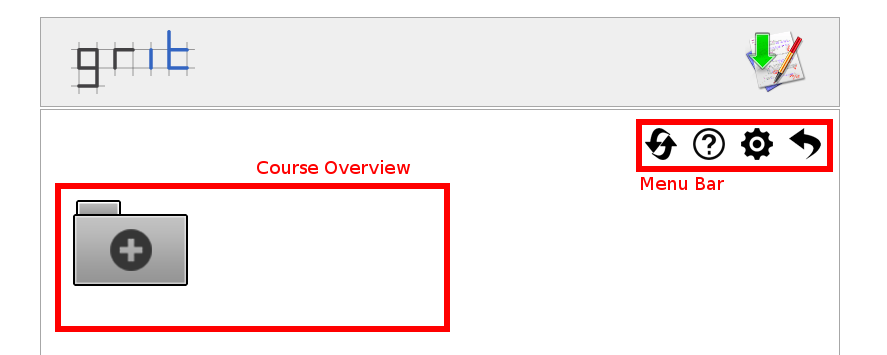
\includegraphics[width=.6\textwidth]{pictures/home.png}
	\end{center}
	Before you start creating new courses you should read section \ref{dataSourceSpecific} because you may need to fulfill external requirements. Now you will need to create a course. For that click on the
        folder with the plus sign.
	\begin{center}
          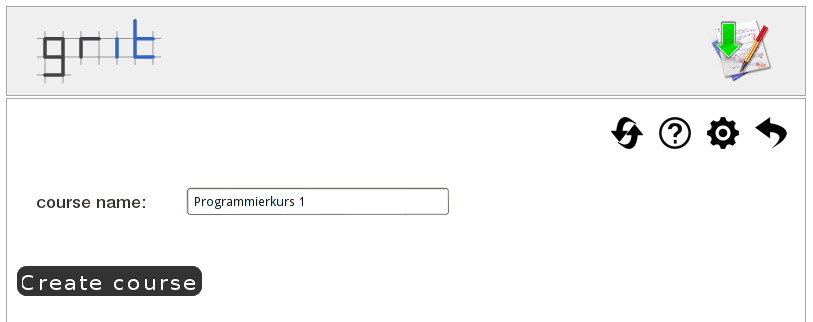
\includegraphics[width=.55\textwidth]{pictures/create_course.png}
	\end{center}
	You will be prompted to enter the course name, after that
        click on {\tt Create course}. The created course will now be
        visible in the overview.
	\begin{center}
          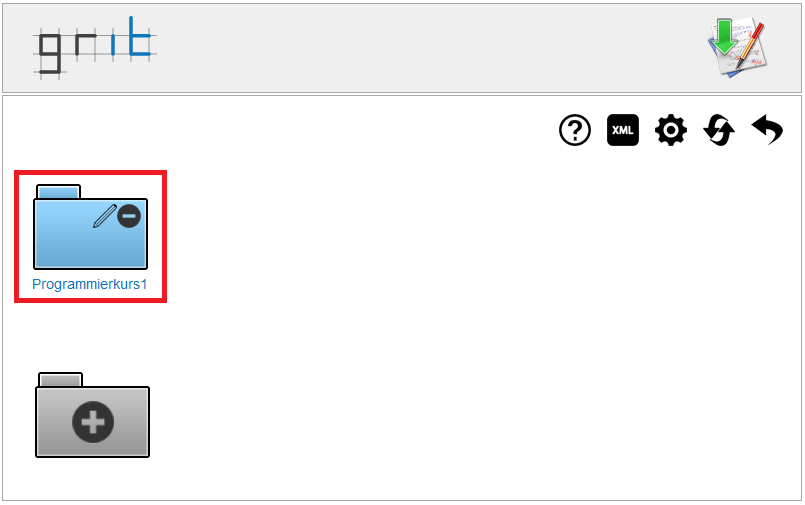
\includegraphics[width=.55\textwidth]{pictures/created_course.png}
	\end{center}For creating an exercise we will first need to set
        up a connection so \product{} knows where to get the students'
        submissions from. For that click on the "gear wheel" symbol in
        the menu bar. You get now presented the connection overview.
	\begin{center}
          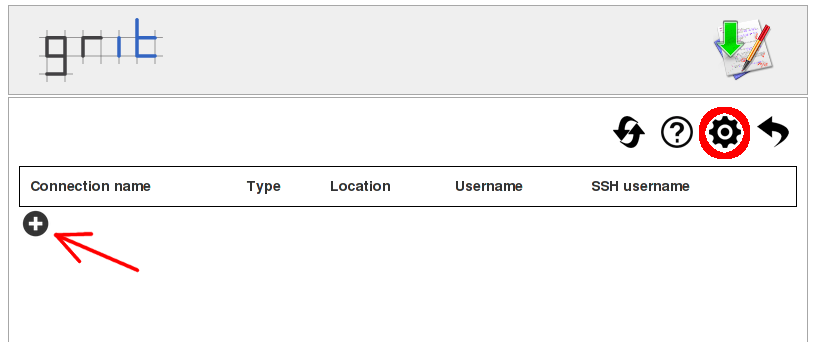
\includegraphics[width=.55\textwidth]{pictures/connection_overview.png}
	\end{center}
	To add a new one click on the plus sign. You will get to a
        form where you can enter the connection information:
	\begin{description}
        \item[Connection Name:] Name for you to identify the
          connection.
        \item[Connection Type:] Either SVN or Mail is
          supported by \product{} \version.
        \item[Location:] The {\tt url} of the root folder where the
          submissions will be. The root folder has to contain the \texttt{students.txt}
        \item[Username:] The name of the SVN account.
        \item[Password:] The password for the SVN or Mail
          account.
        %\item[ssh Username:] If you are setting up an ILIAS
         % connection, enter the account's user name which is being
          %used to copy files from the ILIAS machine.
        %\item[ssh Key-File:] The file containing the key which is used
          %to authenticate the ssh connection with the ILIAS machine.
        \item[Structure:] The strucure that \product{} will encounter
          so it knows where to get the submission. For more see
          Section \ref{structure}.
	\end{description}
	\begin{center}
          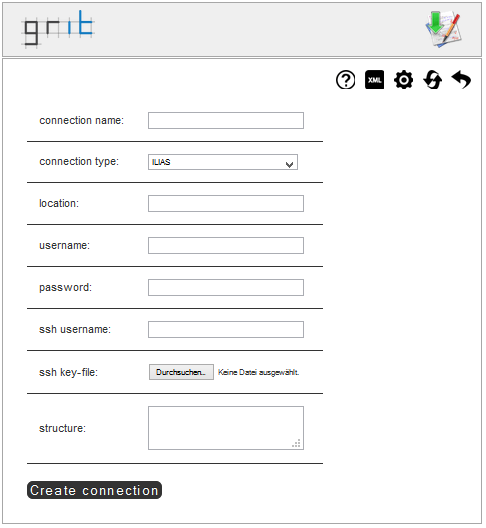
\includegraphics[width=.55\textwidth]{pictures/create_connection.png}
	\end{center}
	At the end click on {\tt Create Connection}. And you will see
        the created Connection in the overview.
	\begin{center}
          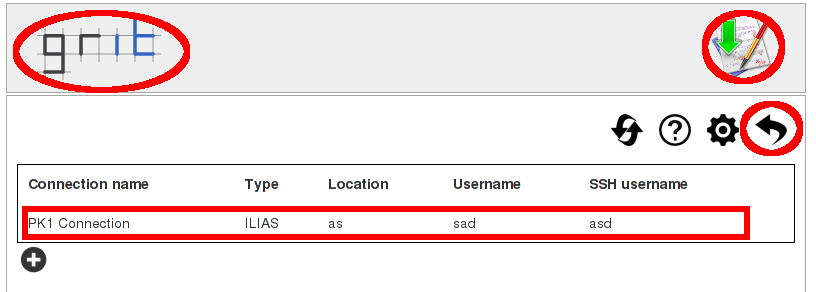
\includegraphics[width=.55\textwidth]{pictures/connection_overview2.png}
	\end{center}
	Now you go back to the course overview. Either by clicking the
        "back arrow" or by clicking the \product{} logo. Now click on
        your created course and you will see the exercise overview.
	\begin{center}
          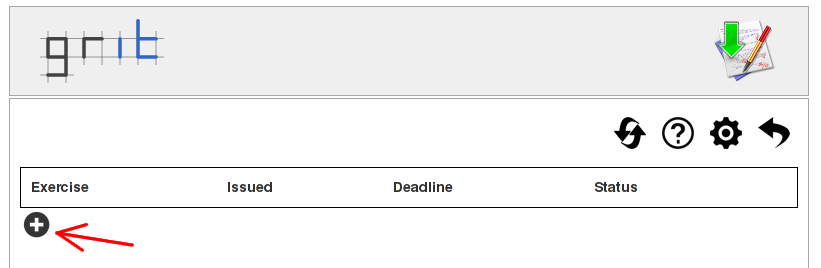
\includegraphics[width=.55\textwidth]{pictures/exercise_overview.png}
	\end{center}
	Similar to the connection overview you can now create a new
        exercise by clicking the plus button and again will be
        prompted a form:
	\begin{description}
        \item[Exercise Name:] The name of the Exercise that will also
          be printed on the output document (i.e. Exercise 1/Übung 1).
        \item[Language:] The programming language for the
          Exercise. Java, C/C++ and Haskell are supported as of
          \product{} \version.
        \item[Start at:] The date the exercise gets handed out to the
          students.
        \item[Deadline:] The date when the students must have
          submitted their submissions.
        \item[Connection to use:] Here you will select the connection,
          previously created, to be used with the exercise.
        \item[Unit Test file:] The (optional) file that contains Unit
          Tests to test for. Only JUnit is supported by \product{}
          \version.
	\end{description}
Please mind that the fetching periods (the time interval between two fetches) have to fit into the interval
between start time and deadline. So if you create an exercise e.g.
between 10:00 and 18:00, the fetching period must not be 45 minutes
because then the last fetch will be 15 minutes past the deadline. 
Also you should create the exercise \emph{before} the start time, 
since otherwise the fetching period will be counted from the creation time.
	\begin{center}
          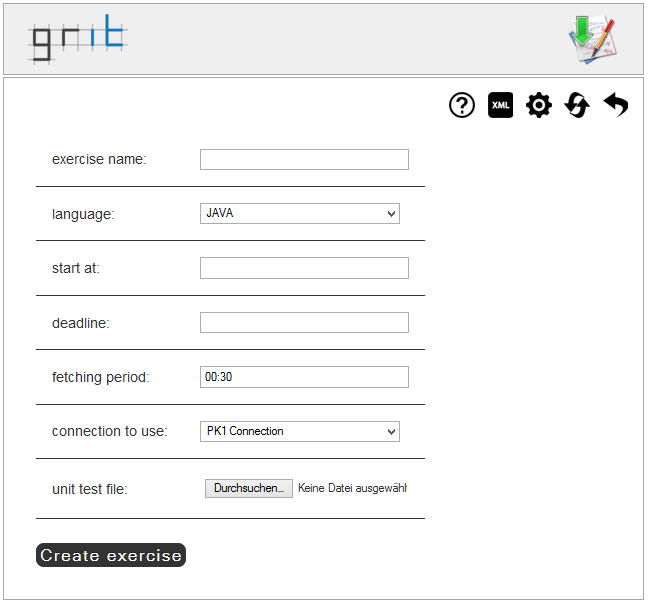
\includegraphics[width=.55\textwidth]{pictures/create_exercise.png}
	\end{center}
	Now you can click {\tt create exercise} and you will see the
        just created exercise in the overview. If you setting made are
        correct everything is set up now and you can wait for the
        deadline. If you made some error you can click the pencil
        symbol to the right of the exercise entry and change the
        settings.
	\begin{center}
          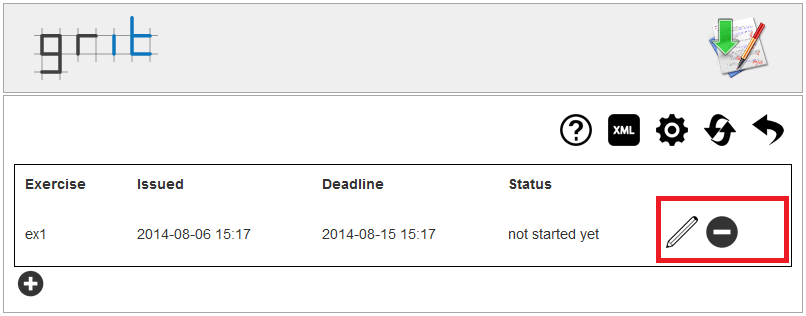
\includegraphics[width=.55\textwidth]{pictures/exercise_overview2.png}
	\end{center}
	Finally the end of the deadline we will process the
        submissions and when finished an additional symbol will be
        visible next to the exercise entry: With that you can download
        the PDF Document containing the students submission, the
        compiler output and - if existing - the test results.

	\section{Setting up a submission structure}\label{structure}
        In order to be able to correctly match student submission
        files to students in SVN repositories, \product{} needs to
        know the structure of the directory tree it is supposed to
        look at. For this purpose you need to enter a comma separated
        list of regular expressions which match the path \product{}
        needs to traverse to find submissions. The special tags
        \texttt{TOPLEVEL} and \texttt{SUBMISSION} indicate the
        repository root and the submission level respectively.

        For example, your repository might have two folders at its
        root: \texttt{exercise/} and \texttt{lecture/}. While the
        latter contains no submissions, \texttt{exercise/} contains a
        folder for each student: \texttt{stud01/}, \texttt{stud02/},
        \texttt{stud03/} and so on. Each of these students has a
        folder for each exercise: \texttt{ex01/}, \texttt{ex02/},
        \texttt{ex03/} and so on.

        In order to tell \product{} to look in a specific folder(e.g. \texttt{ex01})
        you would specify the following list:

        \begin{lstlisting}
          TOPLEVEL
          exercise
          stud[0-9][0-9]
          ex01
          SUBMISSION
\end{lstlisting}

        \texttt{TOPLEVEL} stands for the root of the repository. Then
        \product{} will only look at the \texttt{exercise} folder. In
        there, all folders from \texttt{stud01} upto \texttt{stud99}
        will be inspected. In each student folder \product{} looks at the folder ex01. From
        here the system will retrieve the current submission. With the regular expression as seen above you can have up to 99 student folders. If you need more, you just need to add  \texttt{[0-1]} between \texttt{stud} and \texttt{[0-9]}.
        
	\section{Configuration}\label{config} 
		The config file contains important data for the server, the mail 			notification and the admin account. This information is stored in 		an .xml file located at \texttt{config/config.xml}. If there is 			no config present at boot the standart failsafe config will be 				loaded. This config looks like this:
		\newpage
		\begin{lstlisting}
		<?xml version="1.0" encoding="UTF-8" standalone="no"?>
		<config>
			<server>
				<port value="8080"/>
			</server>
			<email>
				<auth password="" adress="" host=""/>
			</email>
			<admin>
				<user name="username" email="" password="password"/>
			</admin>
		</config>
	    \end{lstlisting}		   
       	The structure consists of the following items:
       	\begin{description}
        \item[<config>:] Wrapper tag which specifies when the config 					starts and when it ends.
        \item[<server>:] Holds info about the server.
        \item[<port>:] The port the server is running on.
        \item[<email>:] Holds info about the email account where the							notification mails are send from.
        \item[<auth>:] All relevant authentication info for the mail account. The password, the mail address and the SMPT host server(e.g. smtp.gmail.com).
        \item[<admin>:] Holds info about the admin account.
        \item[<user>:] The data with which you want to log into the website and the email the admin want to get notifications on.
		\end{description}
		In order to customize the config you just change the values between the quotation marks. To do so please use the respective edit xml function on the webinterface. After the configuration was changed the system needs to be rebooted. This will be done automatically in the edit xml function. You should especially consider this if you changed the config file without the edit xml function on the webinterface.
		
		\section{E-Mail transmission function}
The e-mail sending function for GRIT allows to set up the system so that e-mails will be sent automatically if any number of the following conditions are complied:
\begin{itemize}
\item The file which is delivered by the student is not plausible, i.e the file extension doesn't conform with the required one

\item The file which is delivered by the student doesn't compile
\end{itemize}

If the SVN-Submission system is used as Connection-Type e-mails will also be sent automatically if any number of the following conditions are complied:
\begin{itemize}
\item The student hasn't committed anything 12 hours before the deadline is expired

\item The student hasn't committed anything 6 hours before the deadline is expired
\end{itemize}

\subsection*{Establishment of e-mail transmission function}
This section explains how to set up the e-mail transmission function.\\
Therefore you have to press the button called "XML" of the web interface.
\begin{center}
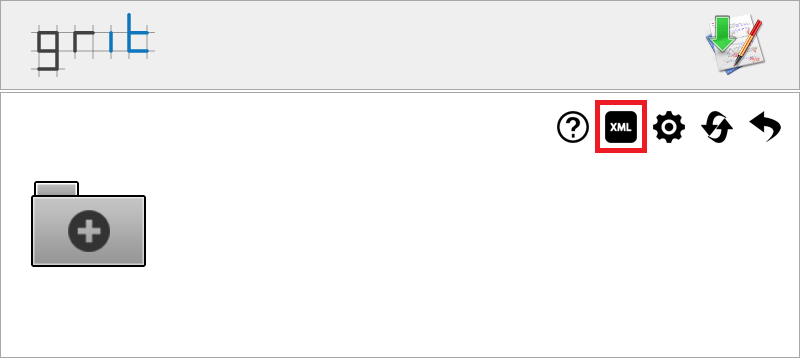
\includegraphics[scale=0.55]{pictures/home_xml-marked.png} 
\end{center}

Thereupon it appears a warning that you have to be carefully when you want to change the XML-File. 
\begin{center}
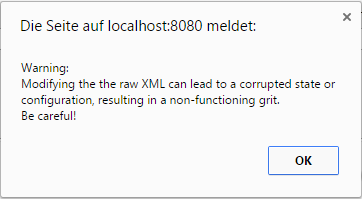
\includegraphics[scale=0.55]{pictures/warning_xml.png} 
\end{center}

By pressing the OK-Button you get to the actual XML-Configuration page:
\begin{center}

\includegraphics[scale=0.55]{pictures/xml.png}
\end{center}

To set up the e-mail transmission function you need only the config-field:
\begin{center}
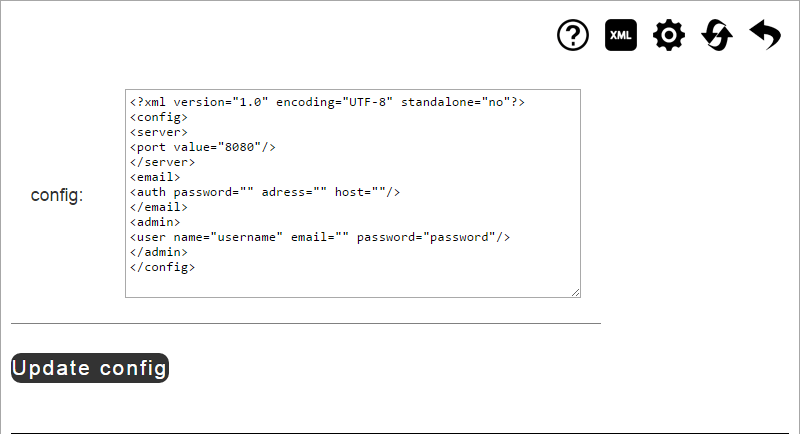
\includegraphics[scale=0.55]{pictures/config_full.png} 
\end{center}

At the config-field the following fields are only important:\\
<email>
\begin{itemize}
\item auth password="PasswordForTheMailsendingAccount"\\
e.g.: auth password="password"

\item adress="MailsendingAddress"\\
e.g.: adress="testaccount@gmail.com"

\item host="MailsendingHost"\\
e.g.: host="smtp.gmail.com"
\end{itemize}
<admin>
\begin{itemize}
\item email="MailaddressOfAdmin"\\
This is the e-mail-address to which GRIT sends an e-mail to, as soon as the report-pdf is ready for download.\\
e.g.: email="adminemail@uni-konstanz.de"
\end{itemize}

\section{E-Mail Submission system}
The e-mail submission system allows to set up GRIT so that students are able to submit their solutions by e-mail.

\subsection*{Establishment of the e-mail submission system}
To set up the e-mail submission system you have to choose the "Connection type" "EMAIL" in a new connection. For this you have to press the button on the web interface which looks like a gear.
\begin{center}
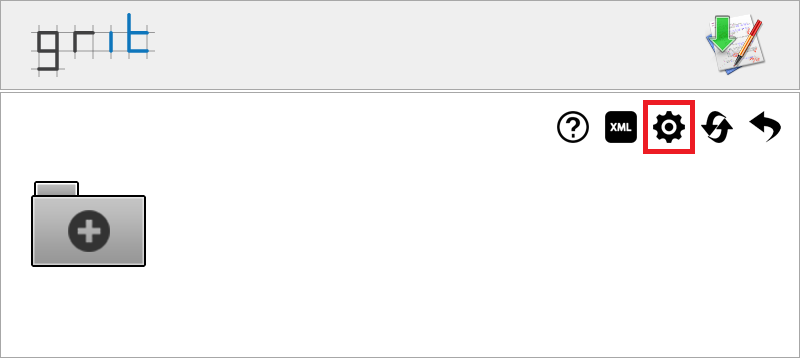
\includegraphics[scale=0.55]{pictures/home_connection-marked.png} 
\end{center}

After this there appears the connection-interface on the web interface. There you have to press the button which looks like a circled plus symbol to set up a new connection:
\begin{center}
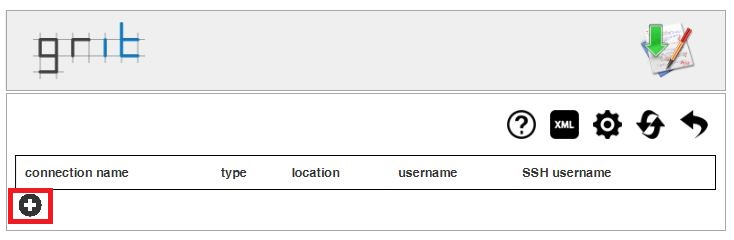
\includegraphics[scale=0.55]{pictures/connection.JPG} 
\end{center}

Now appears the standard-entry mask:
\begin{center}
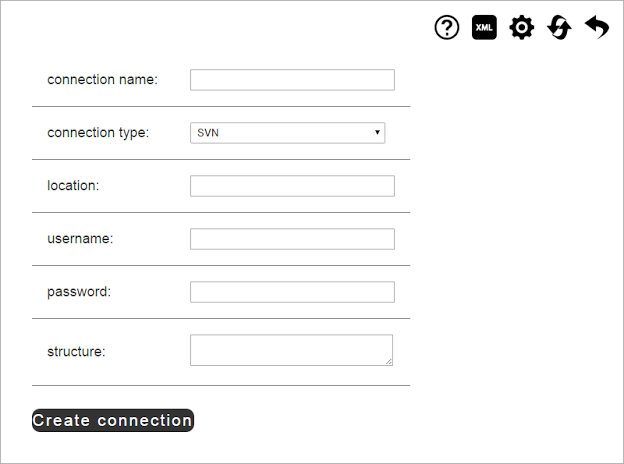
\includegraphics[scale=0.55]{pictures/createNewConnectionSvn.png} 
\end{center}

There you have to set up the "Connection-Type" to "MAIL". Therefore only the necessary input fields for the e-mail submission system are visible:
\begin{center}
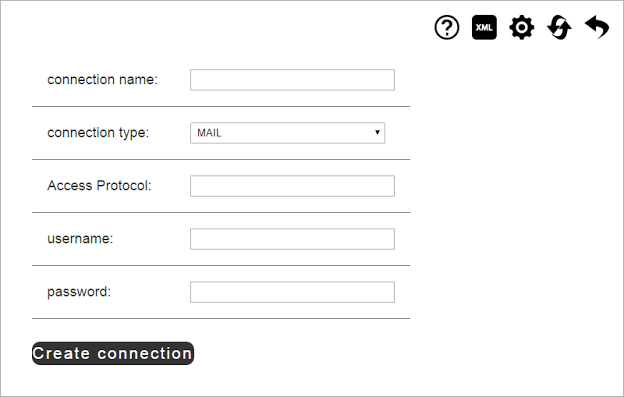
\includegraphics[scale=0.55]{pictures/createNewConnectionMail.png} 
\end{center}

Explanation of the fields:
\begin{itemize}
\item connection name: The name which identifies this connection.\\
e.g.: EMAIL

\item connection type: On which way the submission system fetches the submissions. Either "SVN", which is the standard type or "MAIL", which is selected in this case.

\item Access Protocol: The network protocol of the used e-mail account\\
Please notice that the network protocol should be able to access e-mails received by the e-mail-server\\
e.g.: imap.gmail.com

\item username: The e-mail-address to which the students will send their submissions.\\
e.g.: git@gmail.com

\item password: The password for the e-mail-account
\end{itemize}

       \section{Data Source Specific Requirements}\label{dataSourceSpecific} 
        There are some things you need to consider when creating courses and exercises.
%       \subsection{Ilias}
%       If you create a new course witch will be using an ILIAS connection for an exercise you need to meet some requirements. At first the mapping from \product{} to ILIAS is that courses in \product{} resemble exercises in ILIAS and exercises in \product{} resemble assignments in ILIAS. This is due to the internal database schema of the ILIAS data management. Now you have to make sure that before you create a new course or a new exercise in \product{} this courses and exercises already exist in ILIAS. If not fetching will not work properly. They also need to have exactly the same name. For example:\\\\
%	    \begin{tabular}{c c | c c}
%	    GRIT: 				&		& ILIAS:				& \\\hline
%	    Course: 			&PK1	& Exercise: 			&PK1\\
%	    Exercises of PK1:	&ex1	& Assignments of PK1:	& ex1\\
%	    					&ex2	&						& ex2
%\end{tabular}	 \\\\
%Furthermore you should ensure that there are no ambiguities in the %name schema of the courses and the exercises so that exercises can be clearly distinguished. For example you should not have two courses with the exact same name.
  	
       \subsection{SVN}
       For SVN you have to make sure to choose a different connection
       for every exercise because the submission structure in the
       connection specifies which exercise you want to fetch from the
       repository.\\
       Besides you should guarantee that the submissions of the students must not contain whitespaces in the file name, otherwise the the submission cannot be evaluated.

       \subsection{Email}
       If you decided to use email submissions, you already have
       specified the email address from which \product{} should fetch
       email submissions. In order for this to work as intended,
       students have to name the email subject according to the
       following formula:

       \[ \texttt{[course name-exercise name]} \]

       E.g. when the course name is "Programmierkurs 1" and the
       exercise name is "1" (for the first exercise), then the
       subject should be \texttt{Programmierkurs 1-1} so \product{} can
       find the submission. Also consider that submissions handed in
       after the dead line are not imported.
       
	\chapter{Frequently asked Questions}
	\begin{enumerate}
        \item \textit{What does \product{} do?}
		
          \product{}  assists you in running a programming course where
          it is required for students to hand in assignments done in
          code. The submissions can be automatically fetched from
          associated repositories and automatically tested. \product{} 
          delivers a well-structured and comprehensive document ready
          to be graded by a corrector as well as overall and detailed
          course statistics.
		
        \item \textit{What does \product{} not do?}
		
          \product{}  integrates between the steps assignment issuance,
          submission and correction. To be precise, it fills the
          formerly manual between submission and correction, as well
          as everything that comes after correction. \product{} does not
          provide facilities to issue assignments, submit them, and,
          certainly cannot correct them.
		
        \item \textit{On what type of machine should I install
            \product?}
		
          It is possible to install \product{} on different Linux systems (It is tested on Ubuntu, Debian and OpenSUSE)
          %with Vagrant on Windows
		
        %\item \textit{Do I need a virtual machine for \product?}
		
         % You do not need a virtual machine if you use a linux operating system.
          %Of course you can still use one.\\
          %If you use an other operating system, you need a VM with a Linux operation system.
          
		
		
        \item \textit{What is the default username and password?}
		
          The default username is {\tt username} and its password is
          {\tt password}.
		
       % \item \textit{What is the {\tt root} password?}
		
        %  The {\tt root} password is {\tt root}
		
        \item \textit{Should I change the predefined passwords of the
            provided VM?}
		
          Yes.
		
%        \item \textit{Is it possible to use a graphical user
%            interface?}
%		
%          If you wish to run \product{} natively or on another virtual
%          machine, you will find the associated requirements in
%          \hyperref[4.3]{Section 3 of Chapter 4}.
		
	\end{enumerate}
	\chapter{Credits}
	\section{Developers Team GRIT}
	\begin{itemize}[label=]
        \item Gabriel Einsdorf
        \item Marvin Gülzow
        \item Eike Heinz
        \item Marcel Hiller
        \item David Kolb
        \item Fabian Marquart
        \item Thomas Schmidt
        \item Stefano Woerner
	\end{itemize}
	\section{Developers Team VARCID}
	\begin{itemize}[label=]
        \item Verena Berg \hfill (Verena.Berg@uni-konstanz.de)
        \item Annelie Bruder \hfill (Annelie.Bruder@uni-konstanz.de)
        \item Robert Schmid \hfill (Robert.Schmid@uni-konstanz.de)
        \item Cedric Sehrer \hfill (Cedric.Sehrer@uni-konstanz.de)
        \item Iris Schmidt \hfill (Iris.Schmidt@uni-konstanz.de)
        \item Dirk Oehler \hfill (Dirk.2.Oehler@uni-konstanz.de)
        \item Onur Cakmak \hfill (Onur.Cakmak@uni-konstanz.de)
	\end{itemize}
	\section{Special Thanks}
	\begin{itemize}[label=]
        \item Arno Scharmann
        \item Dr.-Ing. Ernst de Ridder
        \item Sigmar Papendick
        \item Simone Winkler
        \item Tino Klingebiel
        \item Stefan Brütsch
	\end{itemize}
      \end{document}
